\documentclass[a4paper,10pt,oneside]{book} 
\usepackage{graphicx} % allows you to insert graphic files
\usepackage{courier}
\usepackage{color}
\usepackage[utf8]{inputenc}
\usepackage[italian]{babel}
%\usepackage[latin1]{inputenc}
\usepackage{subfigure}
\usepackage{epigraph}
\setlength{\epigraphwidth}{200pt}
\usepackage{amsfonts}
\usepackage{amsmath}
\usepackage{caption}
\captionsetup[figure]{labelfont=bf}
\captionsetup[table]{labelfont=bf}
\usepackage{indentfirst}
\usepackage{float}
\usepackage{setspace}
\usepackage{listings}
\usepackage{wrapfig}
\usepackage{algorithm}
\usepackage{algpseudocode}
\usepackage{pifont}




\frenchspacing
\onehalfspacing

\definecolor{lightgray}{rgb}{.9,.9,.9}
\definecolor{darkgray}{rgb}{.4,.4,.4}
\definecolor{purple}{rgb}{0.65, 0.12, 0.82}
\lstdefinelanguage{GLSL}
{
sensitive=true,
morekeywords=[1]{
attribute, const, uniform, varying,
layout, centroid, flat, smooth,
noperspective, break, continue, do,
for, while, switch, case, default, if,
else, in, out, inout, float, int, void,
bool, true, false, invariant, discard,
return, mat2, mat3, mat4, mat2x2, mat2x3,
mat2x4, mat3x2, mat3x3, mat3x4, mat4x2,
mat4x3, mat4x4, vec2, vec3, vec4, ivec2,
ivec3, ivec4, bvec2, bvec3, bvec4, uint,
uvec2, uvec3, uvec4, lowp, mediump, highp,
precision, sampler1D, sampler2D, sampler3D,
samplerCube, sampler1DShadow,
sampler2DShadow, samplerCubeShadow,
sampler1DArray, sampler2DArray,
sampler1DArrayShadow, sampler2DArrayShadow,
isampler1D, isampler2D, isampler3D,
isamplerCube, isampler1DArray,
isampler2DArray, usampler1D, usampler2D,
usampler3D, usamplerCube, usampler1DArray,
usampler2DArray, sampler2DRect,
sampler2DRectShadow, isampler2DRect,
usampler2DRect, samplerBuffer,
isamplerBuffer, usamplerBuffer, sampler2DMS,
isampler2DMS, usampler2DMS,
sampler2DMSArray, isampler2DMSArray,
usampler2DMSArray, struct},
morekeywords=[2]{
radians,degrees,sin,cos,tan,asin,acos,atan,
atan,sinh,cosh,tanh,asinh,acosh,atanh,pow,
exp,log,exp2,log2,sqrt,inversesqrt,abs,sign,
floor,trunc,round,roundEven,ceil,fract,mod,modf,
min,max,clamp,mix,step,smoothstep,isnan,isinf,
floatBitsToInt,floatBitsToUint,intBitsToFloat,
uintBitsToFloat,length,distance,dot,cross,
normalize,faceforward,reflect,refract,
matrixCompMult,outerProduct,transpose,
determinant,inverse,lessThan,lessThanEqual,
greaterThan,greaterThanEqual,equal,notEqual,
any,all,not,textureSize,texture,textureProj,
textureLod,textureOffset,texelFetch,
texelFetchOffset,textureProjOffset,
textureLodOffset,textureProjLod,
textureProjLodOffset,textureGrad,
textureGradOffset,textureProjGrad,
textureProjGradOffset,texture1D,texture1DProj,
texture1DProjLod,texture2D,texture2DProj,
texture2DLod,texture2DProjLod,texture3D,
texture3DProj,texture3DLod,texture3DProjLod,
textureCube,textureCubeLod,shadow1D,shadow2D,
shadow1DProj,shadow2DProj,shadow1DLod,
shadow2DLod,shadow1DProjLod,shadow2DProjLod,
dFdx,dFdy,fwidth,noise1,noise2,noise3,noise4,
EmitVertex,EndPrimitive},
morekeywords=[3]{
gl_VertexID,gl_InstanceID,gl_Position,
gl_PointSize,gl_ClipDistance,gl_PerVertex,
gl_Layer,gl_ClipVertex,gl_FragCoord,
gl_FrontFacing,gl_ClipDistance,gl_FragColor,
gl_FragData,gl_MaxDrawBuffers,gl_FragDepth,
gl_PointCoord,gl_PrimitiveID,
gl_MaxVertexAttribs,gl_MaxVertexUniformComponents,
gl_MaxVaryingFloats,gl_MaxVaryingComponents,
gl_MaxVertexOutputComponents,
gl_MaxGeometryInputComponents,
gl_MaxGeometryOutputComponents,
gl_MaxFragmentInputComponents,
gl_MaxVertexTextureImageUnits,
gl_MaxCombinedTextureImageUnits,
gl_MaxTextureImageUnits,
gl_MaxFragmentUniformComponents,
gl_MaxDrawBuffers,gl_MaxClipDistances,
gl_MaxGeometryTextureImageUnits,
gl_MaxGeometryOutputVertices,
gl_MaxGeometryOutputVertices,
gl_MaxGeometryTotalOutputComponents,
gl_MaxGeometryUniformComponents,
gl_MaxGeometryVaryingComponents,gl_DepthRange},
morecomment=[l]{//},
morecomment=[s]{/*}{*/},
morecomment=[l][keywordstyle4]{\#},
\lstset{
language=GLSL,
backgroundcolor=\color[rgb]{0.95, 0.95, 0.95},
tabsize=2,
rulecolor=,
basicstyle=\scriptsize,
upquote=true,
aboveskip={1.5\baselineskip},
columns=fixed,
showstringspaces=false,
extendedchars=true,
breaklines=true,
prebreak = \raisebox{0ex}[0ex][0ex]{\ensuremath{\hookleftarrow}},
frame=single,
showtabs=false,
showspaces=false,
showstringspaces=false,
identifierstyle=\ttfamily,
keywordstyle=\color[rgb]{1.0,0,0},
keywordstyle=[1]\color[rgb]{0,0,0.75},
keywordstyle=[2]\color[rgb]{0.5,0.0,0.0},
keywordstyle=[3]\color[rgb]{0.127,0.427,0.514},
keywordstyle=[4]\color[rgb]{0.4,0.4,0.4},
commentstyle=\color[rgb]{0.133,0.545,0.133},
stringstyle=\color[rgb]{0.639,0.082,0.082},
}
}



\lstdefinelanguage{JavaScript}{
  keywords={typeof, new, true, false, catch, function, return, null, catch, switch, var, if, in, while, do, else, case, break},
  keywordstyle=\color{blue}\bfseries,
  ndkeywords={class, export, boolean, throw, implements, import, this},
  ndkeywordstyle=\color{darkgray}\bfseries,
  identifierstyle=\color{black},
  sensitive=false,
  comment=[l]{//},
  morecomment=[s]{/*}{*/},
  commentstyle=\color{purple}\ttfamily,
  stringstyle=\color{red}\ttfamily,
  morestring=[b]',
  morestring=[b]"
}

\lstset{
   language=JavaScript,
   backgroundcolor=\color{lightgray},
   extendedchars=true,
   basicstyle=\footnotesize\ttfamily,
   showstringspaces=false,
   showspaces=false,
   numberstyle=\footnotesize,
   numbersep=9pt,
   tabsize=2,
   breaklines=true,
   showtabs=false,
   captionpos=b
}

\begin{document}
\begin{titlepage}
\begin{center}



\centering


\includegraphics[width=1\textwidth]{img/logo.jpg}


Dipartimento di Informatica
\vspace{30pt}

CORSO DI LAUREA MAGISTRALE IN INFORMATICA
\vspace{30pt}


PROGETTO DI GPU COMPUTING
\bigskip

{\huge\textbf{Parallelizzazione dell'algoritmo Advanced Encryption Standard (AES) su architettura CUDA}}

\vspace{20pt}


\centering

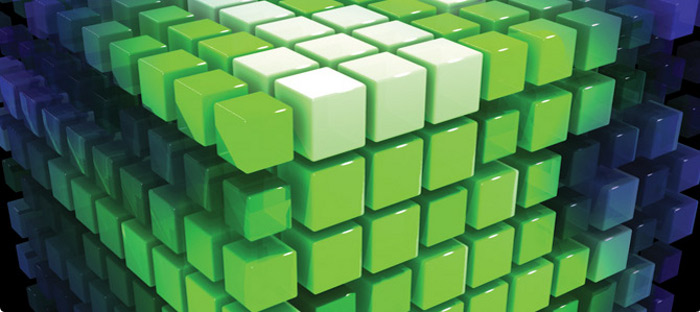
\includegraphics[width=1\textwidth]{img/cudablock.jpg}
\bigskip



\vspace{20pt}

\begin{tabular}{p{230pt}l}
\textit{A cura di} & \textit{Docente} \\
\textbf{Andrea Ceccarelli} & \textbf{Giuliano Grossi}
\\
\textbf{Tommaso Celata}

\end{tabular}
\vspace{25pt}

Anno Accademico 2015/2016
\end{center}
\end{titlepage}



\tableofcontents

\chapter{Introduzione}
Il progetto da noi realizzato si pone l'obiettivo di verificare i vantaggi che l'architettura CUDA può portare nella parallelizzazione di algoritmi che presentano una sostanziosa parte seriale che può essere eseguita parallelamente. Per tale motivo si è scelto l'algoritmo Advanced Encryption Standard \textbf{(AES)} che cifra stati di dimensione fissa senza concatenare i risultati tra loro dandoci la possibilità di ottenere un buon livello di parallelizzazione.

\paragraph{}In una prima fase si è implementato l'algoritmo in linguaggio c verificandone la corretta esecuzione tramite vettori di test trovati online, poi si è modificato il codice per adattarsi e sfruttare l'architettura \textbf{CUDA}. Una prima implementazione non è stata sufficiente per ottenere dei vantaggi rispetto alla versione c, questo dovuto al fatto che venivano lanciati \textbf{troppi kernel} che creando un collo di bottiglia rendevano inutile il vantaggio portato dalla parallelizzazione. Andando avanti con le varie versioni si è diminuito sostanzialmente il numero di kernel lanciati arrivando ad ottenere buoni risultati.

\paragraph{} Spiegheremo quindi le caratteristiche delle varie versioni implementate concentrandoci sull'argomento \textbf{parallelizzazione} e su quali vantaggi (o svantaggi) si sono ottenuti da una versione all'altra.
\chapter{Advanced Encryption Standard (AES)}

\section{Caratteristiche}
Sviluppato dai due crittografi belgi Joan Daemen e Vincent Rijmen l'Advanced Encryption Standard (AES), conosciuto anche come Rijndael, di cui più propriamente è una specifica implementazione, è un algoritmo di cifratura a blocchi utilizzato come standard dal governo degli Stati Uniti d'America. 

\paragraph{}
Data la sua sicurezza e le sue specifiche pubbliche si presume che in un prossimo futuro venga utilizzato in tutto il mondo come è successo al suo predecessore, il Data Encryption Standard (DES) che ha perso poi efficacia per vulnerabilità intrinseche. AES è stato adottato dalla National Institute of Standards and Technology (NIST) e dalla US FIPS PUB nel novembre del 2001 dopo 5 anni di studi, standardizzazioni e selezione finale tra i vari algoritmi proposti.

\subsection{ La chiave di sessione}
AES  usa un \textbf{key schedule} per espandere una chiave primaria corta in un certo numero di chiavi di \textbf{ciclo} differenti. 

\subsection{Lo stato}
AES opera utilizzando matrici di 4x4 byte chiamate \textbf{stati}. Quando l'algoritmo ha blocchi di 128 bit in input, la matrice di stato ha 4 righe e 4 colonne; se il numero di blocchi in input diventa di 32 bit più lungo, viene aggiunta una colonna allo stato, e così via fino a 256 bit. In pratica, si divide il numero di bit del blocco in input per 32 e il quoziente specifica il numero di colonne.

\section{Descrizione dell'algoritmo}
L'algoritmo sfrutta diverse funzioni che modificano i valori della matrice di stato mantenendone però la dimensione. Le singole funzioni vengono poi ripetute in un certo ordine per costruire l'algoritmo vero e proprio.

\subsection{Descrizione ad alto livello}
KeyExpansions—round keys are derived from the cipher key using Rijndael's key schedule. AES requires a separate 128-bit round key block for each round plus one more.
InitialRound
AddRoundKey—each byte of the state is combined with a block of the round key using bitwise xor.
Rounds
SubBytes—a non-linear substitution step where each byte is replaced with another according to a lookup table.
ShiftRows—a transposition step where the last three rows of the state are shifted cyclically a certain number of steps.
MixColumns—a mixing operation which operates on the columns of the state, combining the four bytes in each column.
AddRoundKey
Final Round (no MixColumns)
SubBytes
ShiftRows
AddRoundKey.

\begin{enumerate}
\item \textbf{KeyExpansions} La chiave di cifratura viene espansa dal key schedule per generare una chiave più grande contenente tutte le chiavi di ciclo.
\item \textbf{Round iniziale}
\begin{enumerate}
\item \textit{AddRoundKey} Ogni byte dello stato viene combinato con il byte corrispondente della chiave di ciclo tramite uno XOR
\end{enumerate}
\item \textbf{Rounds}
\begin{enumerate}
\item \textit{SubBytes} Ogni byte viene sostituito con un altro secondo delle tabelle.
\item \textit{ShiftRows} Una trasposizione dove le ultime tre righe dello stato sono shiftate a sinistra un certo numero di volte.
\item \textit{MixColumns} Opera sulle colonne combinandone i byte.
\item \textit{AddRoundKey}
\end{enumerate}
\item \textbf{Round Finale (senza MixColumns)}
\begin{enumerate}
\item \textit{SubBytes}
\item \textit{ShiftRows}
\item \textit{AddRoundKey}
\end{enumerate}
\end{enumerate}




\subsection{AddRoundKey}
Nella fase AddRoundKey, la chiave di sessione viene combinata con lo stato. Per ogni round viene derivata una sottochiave dalla chiave originaria usando il key schedule; ogni sottochiave è della stessa dimensione dello stato. La sottochiave è aggiunta allo stato combinando ogni byte di questo con il corrispondente byte della chiave con uno \textbf{XOR}. 

\begin{figure}[H]
\centering
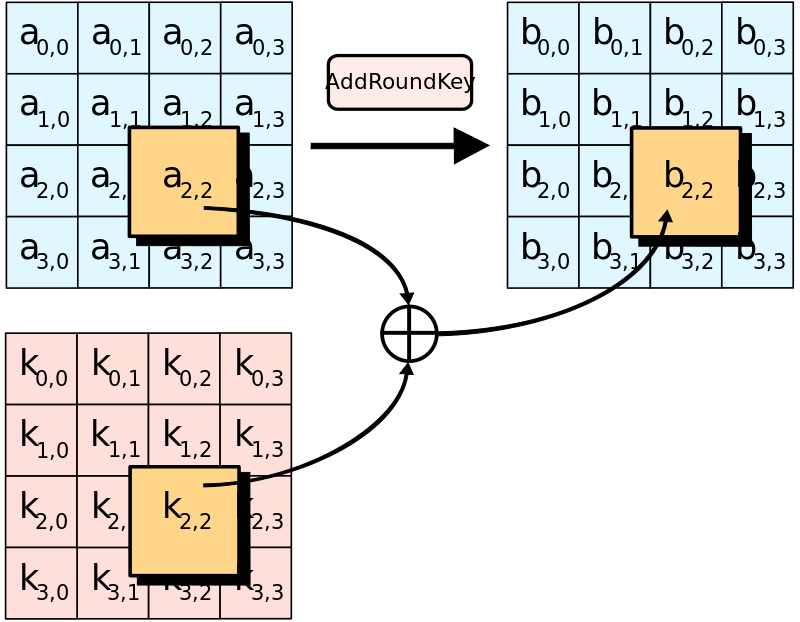
\includegraphics[scale=0.3]{img/addroundkey}
\caption{Nel passaggio AddRoundKeys ogni byte della matrice viene combinato con la sua sottochiave tramite un'operazione di XOR.}
\end{figure}

\subsection{SubBytes}
In SubBytes ogni byte \(a_{i,j}\) della matrice di stato è sostituito con il corrispondente byte di una matrice chiamata  \textbf{S-box}.
\begin{center}
\(b_{i,j} = S(a_{i,j})\)
\end{center}

Questa operazione garantisce la non-linearità della cifratura. 
La S-box utilizzata è derivata da una funzione inversa nel campo finito GF(\(2^8\)), conosciuta per avere delle ottime proprietà di non linearità. Per evitare un potenziale attacco basato sulle proprietà algebriche la S-box è costruita combinando la funzione inversa con una trasformazione affine invertibile. La S-box è stata scelta con cura per non possedere né punti fissi né punti fissi opposti.

\begin{figure}[H]
\centering
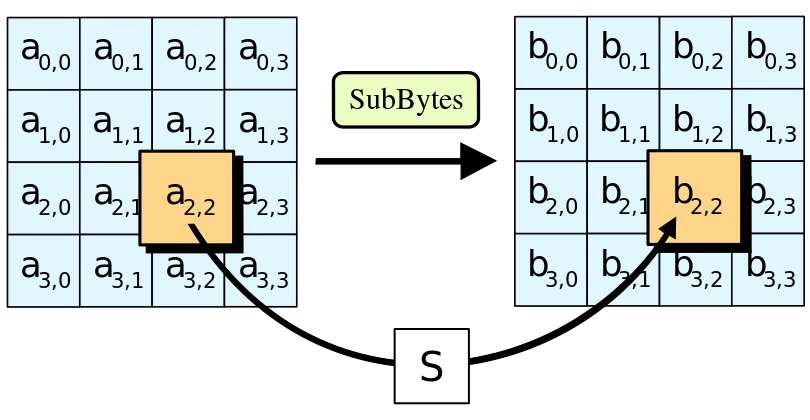
\includegraphics[scale=0.3]{img/subBytes}
\caption{Nel passaggio SubBytes, ogni byte della matrice è sostituito con i dati contenuti nella trasformazione S; \(b_{ij} = S(a_{ij})\).}
\end{figure}

\subsection{ShiftRows}
ShiftRows opera sulle righe dello stato shiftando ciclicamente i byte di ogni riga di un certo offset dipendente dal numero di riga lasciando la prima riga invariata.
Ogni byte della seconda riga è ciclicamente spostato a sinistra di una posizione. Similmente i byte della terza riga sono shiftati ciclicamente a sinistra di due posizioni e quelli della quarta di tre. 

In questo modo l'ultima colonna dei dati in ingresso andrà a formare la diagonale della matrice in uscita. (Rijndael utilizza un disegno leggermente diverso per via delle matrici di lunghezza non fissa.)


\begin{figure}[H]
\centering
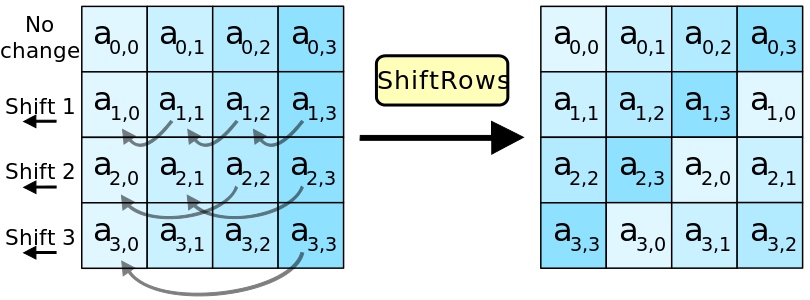
\includegraphics[scale=0.3]{img/shiftRows}
\caption{Nel passaggio ShiftRows, i byte di ogni riga vengono spostati verso sinistra dell'ordine della riga. Vedi figura per i singoli spostamenti.}
\end{figure}

\subsection{MixColumns}
Il passaggio MixColumns prende i quattro byte di ogni colonna e li combina utilizzando una trasformazione lineare invertibile. Utilizzati in congiunzione, ShiftRows e MixColumns provvedono a far rispettare il criterio di confusione e diffusione nell'algoritmo (teoria di Shannon). Ogni colonna è trattata come un polinomio in \(GF(2^8)\) e viene moltiplicata modulo \(x^4+1\) per un polinomio fisso \(c(x)=3x^3+x^2+x+2\).

\begin{figure}[H]
\centering
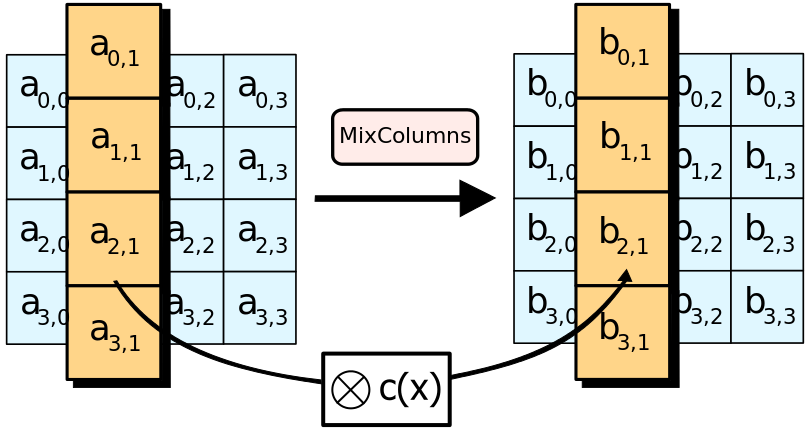
\includegraphics[scale=0.3]{img/mixColumns}
\caption{Nel passaggio MixColumns ogni colonna di byte viene moltiplicata per un polinomio fisso \(c(x)\).}
\end{figure}

\chapter{Architettura CUDA}
\section{Cos'è CUDA}
CUDA ( Compute Unfied Device Architecture) è un architettura hardware creata da NVIDIA e pensata per l’elaborazione parallela che si basa dunque sulla suddivisione di un problema in sottoproblemi e lo svolgimento di ognuno di questi concorrentemente.
Tutto ciò è possibile sfruttando la potenza di calcolo della GPU (unità di elaborazione grafica) che assieme alla CPU permette di rendere molto efficiente in termini di tempo l’esecuzione di molte applicazioni.
Il calcolo parallelo su GPU offre prestazioni senza precedenti caricando porzioni \textbf{compute-intensive} dell'applicazione sulle GPU, mentre la porzione rimanente di codice continua ed eseguire su CPU. Pertanto, le GPU devono operare congiuntamente con le CPU mediante bus PCI-Express

\begin{figure}[H]
\centering
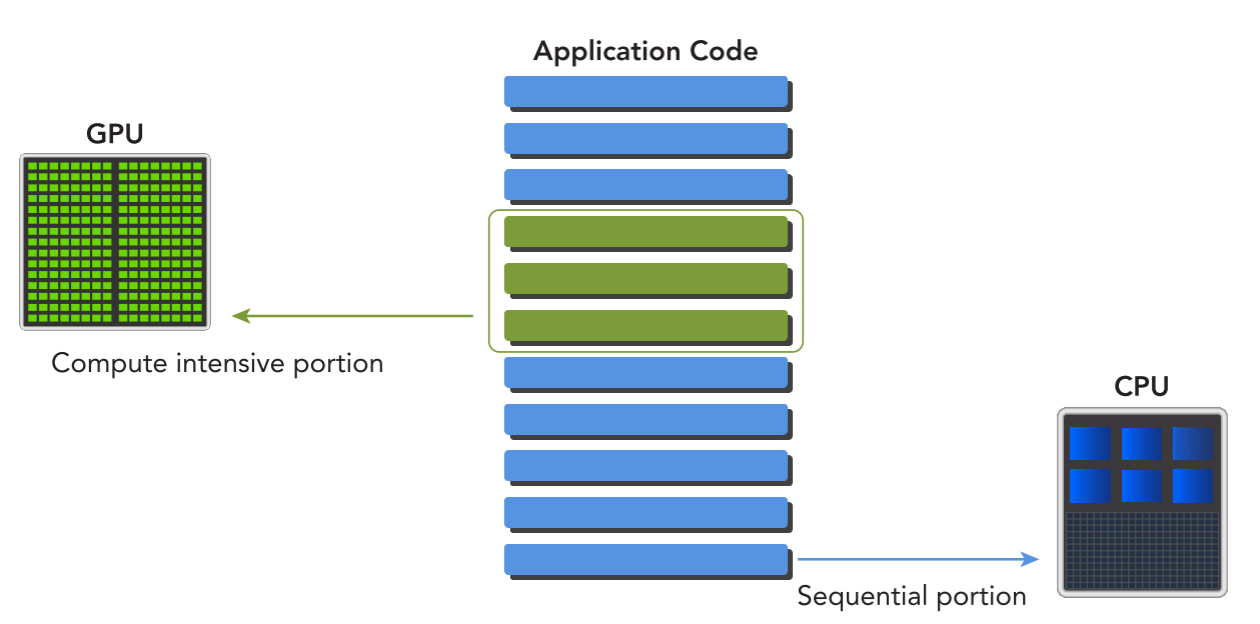
\includegraphics[scale=0.3]{img/cpu-gpu.png}
\caption{Divisione delle operazioni tra GPU e CPU in ambiente CUDA}
\end{figure}

\paragraph{}
Le applicazioni in cui CPU e GPU lavorano insieme consistono di due parti:
\begin{itemize}
\item codice Host
\item codice Device
\end{itemize}


Il codice Host esegue su \textbf{CPUs} e il codice device esegue su \textbf{GPUs}. Il codice CPU è responsabile della gestione dell'ambiente, dell'IO e della gestione dei dati per il device stesso, prima di caricare task intensivi sul device. La GPU è usata per accelerare l'esecuzione di questa porzione di codice basandosi sul parallelismo dei dati. La CPU è ottimizzata per sequenze di operazioni in cui il controllo del flusso è impredicibile; le GPU lo sono per carichi dominati da semplice flusso di controllo.

\begin{figure}[H]
\centering
\includegraphics[scale=0.3]{img/Performancecpu-gpu.png}
\caption{Prestazioni tra GPU e CPU in relazione a grado di parallelismo e quantità dei dati da elaborare.}
\end{figure}
\chapter{Parallelizzazione AES in CUDA}
Per poter ottenere buoni risultati nel campo del GPU Computing c'è bisogno di un algoritmo che ci consenta un sufficiente grado di parallelizzazione.
La scelta di AES infatti non è casuale: basti pensare a come l'algoritmo opera \textbf{indipendentemente} su uno stato o su un altro senza concatenare le due cose e subito ci accorgiamo che consente un alto grado di \textbf{parallelizzazione}.
L'obiettivo del nostro progetto è quindi quello di dimostrare come l'alto grado di parallelizzazione offerta dall'architettura CUDA possa essere utile nell'algoritmo AES. 

\paragraph{Implementazione in C}In una prima fase abbiamo sviluppato l'algoritmo in C per poterlo usare poi come confronto con la versione in CUDA. Sia la versione C che la versione CUDA seguono le seguenti fasi:
\begin{itemize}
\item Lettura del \textbf{plainText}, il testo in chiaro scritto in esadecimale
\item Lettura di una chiave da 16 caratteri esadecimali e generazione di una chiave \textbf{estesa} da 176 sufficente per 11 round
\item Separazione del plainText in stati da 16 elementi.
\item Esecuzione dell'algoritmo su ogni stato
\item Controllo della corretta esecuzione tramite confronto con vettore di test
\item Salvataggio dei risultati per fattore tempo
\end{itemize}

Per quanto riguarda i risultati in fattore tempo questi vengono calcolati comprendendo non solo la fase vera e propria dell'esecuzione di AES ma anche quella di separazione degli stati visto che nel caso GPU questa comprende anche il passaggio dei dati da \textbf{host memory} (memoria centrale) a \textbf{GPU memory}. Abbiamo voluto includere nelle prestazioni questa fase considerando che la memoria è un noto \textit{bottleneck} da considerare.

\section{Prima implementazione in CUDA - Un solo stato}
Una prima implementazione dell'algoritmo in CUDA non considerava una pluralità di stati ma si concentrava solo sulla parallelizzazione delle \textbf{funzioni interne} quali subBytes, addRoundKey ecc...
Purtroppo i risultati furono scoraggianti, infatti nonostante fossimo riusciti a replicare il funzionamento di AES in CUDA verificandone il successo con il vettore di test, i tempi erano di molto peggiori rispetto alla versione C.
\paragraph{Perchè?} Abbiamo pensato che un solo stato non fosse sufficiente per evidenziare un miglioramento nella nostra versione e che questo fosse dovuto proprio a un bottleneck della memoria.

\section{Seconda implementazione in CUDA - Più stati}
Sulla considerazione precedente abbiamo applicato l'algoritmo a più stati contemporaneamente criptando porzioni di testo maggiori e non più limitate a 16 caratteri esadecimali.
In questo modo non solo abbiamo aumentato le dimensioni dei test ma abbiamo anche ottenuto una parallelizzazione più "esterna", in aggiunta a quella già implementata.

\begin{lstlisting}[caption={Versione sequenziale di addROundKey}]
void addRoundKey(uChar** state, int cur_round) {
	for (int i = 0; i < columns; i++) {
		for (int j = 0; j < rows; j++) {
			int val = (cur_round * 16) + ((i * 4) + j);
			state[j][i] = state[j][i] ^ expanded_key[val];

		}
	}
	
	\end{lstlisting}

\begin{lstlisting}[caption={Versione parallela di addROundKey}]
__device__ void addRoundKey(uChar* bufferGPU, int cur_round, uChar* expanded_keyGPU) {
	int Row = blockIdx.y * blockDim.y + threadIdx.y;
	int Col = blockIdx.x * blockDim.x + threadIdx.x;
	int index = Col * M + Row;
	int val = (cur_round * 16) + index;
	bufferGPU[(blockIdx.x*cur_round)+index] = bufferGPU[(blockIdx.x*cur_round)+index] ^ expanded_keyGPU[val];
	


}
\end{lstlisting}


\chapter{Risultati}
\chapter{Considerazioni}
\backmatter
\begin{thebibliography}{}
\bibitem{stornprice}
Kenneth Price , Rainer M. Storn , Jouni A. Lampinen, \textit{Differential Evolution: A Practical Approach to Global Optimization (Natural Computing Series}). Springer-Verlag New York, Inc., Secaucus, NJ, 2005

\end{thebibliography}
\end{document}